\documentclass[a4paper,10pt]{article}

% standard packages
\usepackage[utf8]{inputenc}
\usepackage[english]{babel}
\usepackage{csquotes}
\usepackage{geometry}
\usepackage{graphicx}
\usepackage[textsize=footnotesize]{todonotes}

% This is needed for multiple bib-files
% \usepackage[
% 	sortcites=true,
% 	backend=bibtex,
% 	style=ieee,
% 	defernumbers=true,
% ]{biblatex}
% \addbibresource{references.bib} % The name of your bibliography file

% load macros (section title can be changed here)
% section title macros (can be changed)
\newcommand{\insertProjectFundingSchemeTitle}{Project Funding Scheme:}
\newcommand{\insertProjectShortSummaryTitle}{Short Summary:}

% other macros (do not change)
\makeatletter

\newcommand\projectCode[1]{\renewcommand{\insertProjectCode}{#1}}
\newcommand\insertProjectCode{\@latex@error{No \noexpand\projectCode given}\@ehc}

\newcommand\projectTitle[1]{\renewcommand{\insertProjectTitle}{#1}}
\newcommand\insertProjectTitle{\@latex@error{No \noexpand\projectTitle given}\@ehc}

\newcommand\projectPIs[1]{\renewcommand{\insertProjectPIs}{#1}}
\newcommand\insertProjectPIs{\@latex@error{No \noexpand\projectPIs given}\@ehc}

\newcommand\projectFundingScheme[1]{\renewcommand{\insertProjectFundingScheme}{#1}}
\newcommand\insertProjectFundingScheme{\@latex@error{No \noexpand\projectFundingScheme given}\@ehc}

\newcommand\projectShortSummary[1]{\renewcommand{\insertProjectShortSummary}{#1}}
\newcommand\insertProjectShortSummary{\@latex@error{No \noexpand\projectShortSummary given}\@ehc}

%\newcommand\insertProjectHeader{
%  \noindent\hrulefill\\[.5em]
%  \noindent\llap{\fbox{\bfseries\insertProjectCode}\hspace{1em}}{\Large\bfseries\insertProjectTitle} \\[.5em]
%  PIs: \insertProjectPIs\\
%  \null\hrulefill \\[.5em]
%  \begin{tabular}{@{}ll}
%    {\bfseries\insertProjectFundingSchemeTitle} & \insertProjectFundingScheme \\[.5em]
%    {\bfseries\insertProjectShortSummaryTitle} & \insertProjectShortSummary
%  \end{tabular}\\[.5em]
%  \null\hrulefill
%}

\usepackage{tabularx}

\newcommand\insertProjectHeader{
  \noindent\hrulefill\\[.5em]
  \noindent\llap{\fbox{\bfseries\insertProjectCode}\hspace{1em}}{\Large\bfseries\insertProjectTitle} \\[.5em]
  PIs: \insertProjectPIs\\
  \null\hrulefill \\[.5em]
  \begin{tabularx}{\textwidth}{@{} l X @{}}
    {\bfseries\insertProjectFundingSchemeTitle} & \insertProjectFundingScheme \\[.5em]
    {\bfseries\insertProjectShortSummaryTitle} & \insertProjectShortSummary
  \end{tabularx}\\[.5em]
  \null\hrulefill
}

\makeatother



%%%%%%%%%%%%%%%%%%%%%%%%%%%%%%%%%%%%%%%%%%%%%%%%%%%%%%%%%%%%%%%%%%%%%%%%%%%%%%%%
% PLEASE NOTE THE FOLLOWING LENGTH RESTRICTION:
% - no more than 4 pages (incl. publications). 
% - no more than 8 pages (incl. publications) in the exceptional case that you apply for two positions
%%%%%%%%%%%%%%%%%%%%%%%%%%%%%%%%%%%%%%%%%%%%%%%%%%%%%%%%%%%%%%%%%%%%%%%%%%%%%%%%

\newcommand{\bibfilename}{mrabbrev,mybibfile} % <- replace 'mybibfile' with basename of your bibfile


%%%%%%%%%%%%%%%%%%%%%%%%%%%%%%%%%%%%%%%%%%%%%%%%%%%%%%%%%%%%%%%%%%%%%%%%%%%%%%%%
% FILL OUT PROJECT INFORMATION

%%%%% PROJECT CODE
% Please assign your planned project to one Application Area or Emerging Field of MATH+.
% Code "AA1": Application Area 1 (Life Sciences)
% Code "AA2": Application Area 2 (Materials, Light, Devices)
% Code "AA3": Application Area 3 (Networks)
% Code "AA4": Application Area 4 (Energy and Markets)
% Code "EF1": Emerging Field 1 (Extracting Dynamical Laws from Complex Data)
% Code "EF2": Emerging Field 2 (Digital Shapes)
% Code "EF3": Emerging Field 3 (Model-Based Imaging)
% Code "EF4": Emerging Field 4 (Particles and Agents)
% Code "EF5": Emerging Field 5 (Concepts of Change in Historical Processes)
\projectCode{AA2}

%%%%% PROJECT TITLE
% e.g., Deep learning in Berlin administrations
\projectTitle{Multi Material Electocatalysis II}
%%%%% PIs / Applicants
% Project _heads_ only!
% In case a doctoral researcher is to be selected for a position in the project, 
% applicants must indicate with "*" which PI will act as authorized PhD-supervisor. 
% Form: initial dot lastname, initial dot lastname
\projectPIs{J. Fuhrmann, M. Landstorfer}

%%%%% REQUESTED STAFF
% Please use the following code for the position you request:
% Category A)	Full positions (100% E13) for 2 years, 
% Category B)	75% positions (E13) for 3 years (for projects in AAs and EFs only). 
% If you already know whom you intend to hire, please include the name such as "Category A (Dr. Angela Merkel); Start: 1 JAN 2021"
% In this case, please also include the CV of this person as an additional document in your proposal.
\projectFundingScheme{Category A (Dr. Rüdiger Müller); Start: 1 JAN 2021}

%%%%% SHORT SUMMARY
% Please add a short summary of your project using a maximum of 100 words or 5 lines!!!
\projectShortSummary{Complex, multi-materail electrocatylysts are crucial in many
  applications relevant for the energy transition. Their model based understanding
  will increase the efficiency  and scalability  of electrocatalytic processes.
  Building on the results of the first project period focused on
  thermodynamic equilibrium, modeling an numerical methods  shall be extended to the non-equilibrium case of
  complex surface reactions.
}

%%%%%%%%%%%%%%%%%%%%%%%%%%%%%%%%%%%%%%%%%%%%%%%%%%%%%%%%%%%%%%%%%%%%%%%%%%%%%%%%
% MAIN CONTENT

\begin{document}

\insertProjectHeader


\subsection*{Extended Synopsis of the Proposal}

\paragraph{Background}
% Please include here:
% - Account of the problem
% - Motivation
% - Background
% - State of the art of research in this area
% - Preliminary work by the PIs


% - Account of the problem

The pivotal strategic importance of  technologies based on electrocatalytic reactions
is underlined in  the  recently  approved  National Hydrogen  Strategy of  the  German
Federal  Government. This initiative  grants  hydrogen,  and  in   particular  ``green
hydrogen''  created with  renewable  energy a  strategic  role in  the
decarbonization of the economy as an energy carrier, an energy storage
option, a  sector coupling  technology, a  precursor for  the chemical
industry  and a  means  for  CO2  emission reduction  in  various
industrial  processes. 
As  a part  of this  strategy, the  creation of
hydrogen  from  electrical energy  in  electrolyzers  and the  reverse
process --  the recovery  of electrical energy  from hydrogen  in fuel
cells -- are seen  as indispensable technologies whose development
shall be  supported by  R\&D investments  and market  incentives.
%
Both technologies are based  on electro-catalytic reactions. Production
and utilization  of hydrogen are just  two examples for this  class of
reactions, other  electro-catalytic reactions  are fundamental  in post
lithium  batteries,  material  synthesis  and  other  fields. 

% - Motivation
The main driving forces for the rapid development of these technologies are (i) the synthetization of new electrode and electrolyte materials (e.g. ionic liquids and perovskites) (ii) the fabrication of nano-structured and composite electro-catalyitc surfaces (multi-material catalysts) and (iii) material and operational optimization. Central goal is to reduce cost, the main issue of large scale electro-catalysis due to high amount of expensive raw materials which are yet required (especially Pt and Pd). The Berlin based cluster of excellence UniSysCat, for example, searches for substitutions of these expensive materials.

% - Background
Investigations of electro-catalytic reactions on new materials  
%is one of  the main areas
%of research  in electrochemistry.  These  reactions take place  at the
%interface between  (mostly metallic)  catalysts and  electrolytes.
%They  are investigated  by a
are carried out by a number of  experimental techniques,  e.g.
RRDE    (Rotating   Ring    Disc   Electrode),   
% DEMS   (Differential Electrochemical  Mass  Spectroscopy), 
CV  (Cyclic  Voltammetry),  
STM (Scanning Tunneling Microscopy), 
% EQCM (Electrochemical Quartz Crystal Microbalance), 
SEM (Scanning  Electrochemical Microscopy),
AFM (Atomic Force Microscopy), 
EIS (Electrochemical Impedance Spectroscopy).
% - State of the art of research in this area

In order  to interpret  the experimental  results, and to understand,
predict and optimize electro-catalytic systems, various mathematical models
%on various scales and of
%various  levels of  accuracy 
have to be used. Depending  on the  level of  complexity,
modeling  results  can  be  expressed using  analytic  expressions  or
need to be obtained via numerical simulation.


% Showing the  relevance of mathematical and  numerical modeling, 
Recent research by  internationally leading groups  more and
more focuses  on the  interplay between  mass transport, reactions and the 
electric    field    on   the     nanoscale, resolving double layer effects \cite{lin2019understanding,tan2018double,eden2019modeling,bohra2019modeling}.
%
%The    authors    of
%\cite{lin2019understanding}          and         \cite{tan2018double},
%\cite{eden2019modeling} focus on models and simulation of these processes
%at nanoparticles or homogeneous  (single crystalline) electrodes based
%on     classical    Nernst-Planck     models.    The     authors    of
%\cite{bohra2019modeling} work in the  same direction using generalized
%Nernst-Planck models similar to those derived at WIAS.

All these approaches are based on homogeneous interfaces with no variation in their
spatial  structure. Especially they  do   not  take  into surface inhomogenities, which lead to variations on the electro-chemical activity. 
%heterogeneity   of   the   electrochemical  interfaces   due 
%to   the
%\emph{e.g.} due to a polycrystalline structure  of the catalyst, the restructuring  of the
%catalyst surfaces depending  on various stages of the  reaction or due
%to defects like steps that create spots of increased activity.
%Moreover, these activities are lacking a strategy to upscale the nanoscale
%results to the macrocscale of real experimental or practical devices.

% - Preliminary work by the PIs
WIAS research group  RG7 represented by PI M. Landstorfer is active
in the development of mathematical models for electrochemical systems.
A seminal result is in the derivation of a comprehensive electrolyte model 
%which takes into account finite ion sizes, solvation effects and the influence of pressure.
%This model provides an 
which provides an accurate description of the electrochemical double layer and yields broad accordance to experimental data of single crystal electrodes. % of the double layer differential capacity of single crystal electrodes. % with respect to the applied voltage and
%with respect to the salt concentration.
%layers  and is  able to  predict qualitatively and in the correct quantitative range thedifferential capacity of single crystal electrodes with respect to the applied voltage and
%with respect to the salt concentration. 
Based on this, thermodynamically consistent boundary conditions for electro-chemical reactions at electrode surfaces derived from  surface thermodynamics at the electrode-electrolyte interface have been developed \cite{DGM2013,DGL2014,Landstorfer2016187,landstorfer2017boundary}.

WIAS reserch group RG3 represented by PI J. Fuhrmann contributes to the numerical modeling of electrochemical systems,
including the derivation of a thermodynamically consistent finite volume  method \cite{JF2016} implementing
the model \cite{DGL2014}. A similar discretization approach is used for the simulation
of solide oxide electrolytes \cite{VagnerEtAl2019}. Convergence investigations for different flux
thermodynamically consistent flux expressions of  finite volume
schemes for unipolar drift-diffusion models  have been  performed in \cite{CCFG2020}, see also Fig. \ref{fig:fv}, left. The finite volume method for
ion transport has been coupled to a pressure robust Navier-Stokes solver for electrolyte flow
\cite{FGLMMSpringer2019,FuhrmannEtAlECActa2019}, see also Fig. \ref{fig:fv}, right.
The Julia language allows to utilize forward mode automatic differentiation to significantly reduce the implementation effort for strongly nonlinear problems reducing to reduce code complexity compared to C++ and to allow for easy distribution of the code based on a modern package management system.
The computational  results  in  \cite{CCFG2020,VagnerEtAl2019} have been obtained by the  new Julia package for finite volume methods \cite{VoronoiFVM} developed by the PI.



Recently published work\cite{JES}, supported by Math+ within the project MultECat, provides first results on modeling, simulation and validation of electro-chemical interfaces on polycrystalline materials (see Fig. \ref{fig:JES}). In addition a methodological approach to handle realistic multi-material surfaces was developed, allowing for a stochastic description of polycrystalline surfaces. Additional results on Debye--Hückel theory, concentration dependent susceptibilities, and electrolyte transport are in the final stage of publication. % HIER DIE ARBEITEN IN PREP HIn

%with
%respect to the application of the improved electrochemical double layer
%theory to the case of polycrystalline  electrodes. Based on the assumption of large
%grain sizes compared to the Debye length, characteristic data of the electorchemical double layer,
%like charge, capacitance and potential of zero charge of a polycrystalline electrode can be derived from  the corresponding data
%for the different kinds of grains weighted with their respective surface fraction,
%see Fig. \ref{fig:JES}. 

\begin{figure}
  \centering
  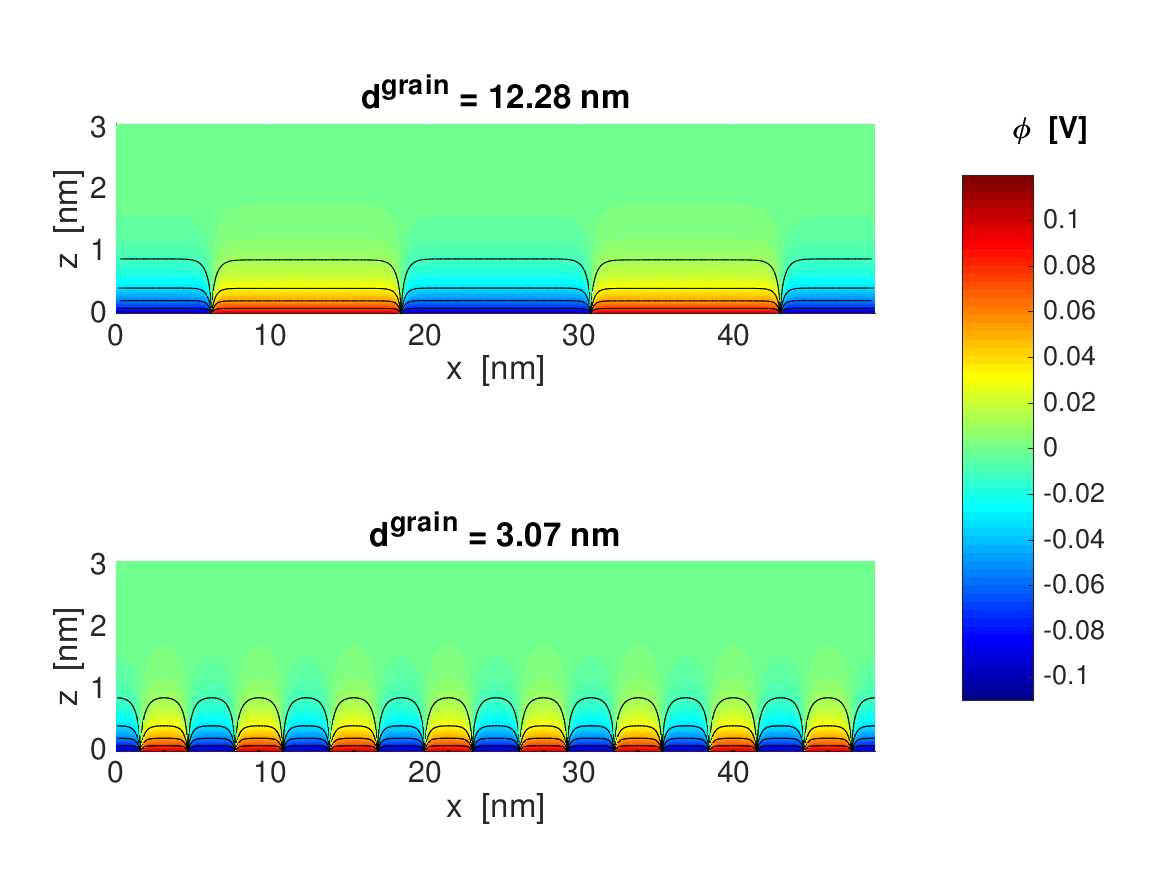
\includegraphics[width=0.45\textwidth]{phi_poly2d_gran.pdf}
  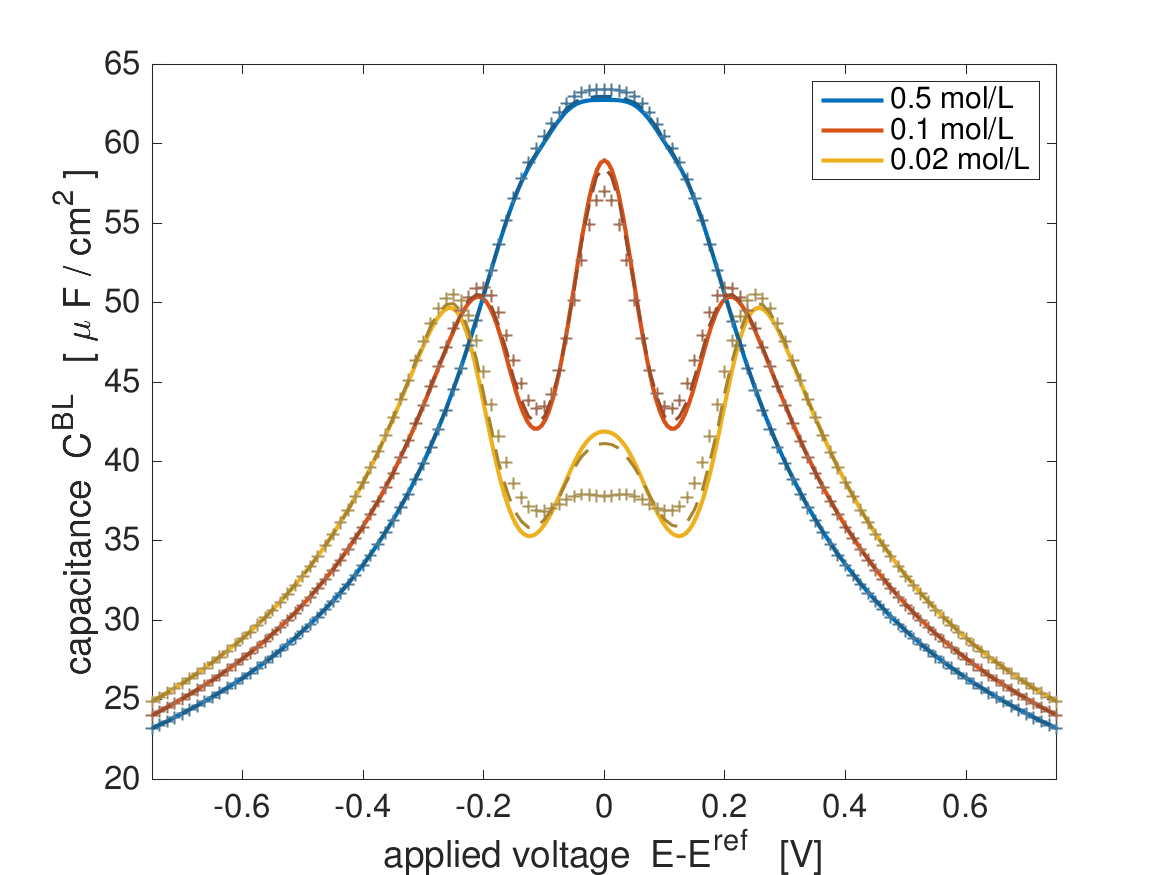
\includegraphics[width=0.45\textwidth]{c_2d_grain.pdf}
  \caption{Left: profile of the electrostatic potential for a bi-crystalline interface with different
    grain sizes.
    Right: double layer capacity curves for different electrolyte concentrations.
    Solid lines (—) refer to the weighted sum of the grain contributions.,
    (+) and dashed (- -) lines mark data obtained from numerical simulations for
    small and large grain sizes, respectively.
 \label{fig:JES}}
\end{figure}

\begin{figure}
  \centering
  \includegraphics[width=0.5\textwidth]{ccfg.pdf}
  \includegraphics[width=0.4\textwidth]{iceo.pdf}
   \caption{Left and mid: time evolution of electorstatic potential and concentration for
  a unipolar Nernst-Planck-Poisson system with volume constraints. The concentrations $c$
  stays in the physical limits $0<c<1$ \cite{CCFG2020}.
  Right: induced charge electroosmotic flow over a floating electrode induced by a lateral
  electric field \cite{FuhrmannEtAlECActa2019}. \label{fig:fv}}
\end{figure}


\paragraph{Goals of the Project and Methodologies}
% Please include here:
% goals
% methodologies
Our recent results on modeling multi-material and polycrystalline metal-electrolyte interfaces are confined to the case of thermodynamic equilibrium without charge transfer reactions. This experimentally validated model framework is our starting point for non-equilibrium thermodynamic modeling of electron transfer reactions at multi-material electrodes coupled to charge transport in an electrolyte, taking into account  effects of polycrystalline interface structure, catalyst surface phase transitions, finite ion sizes, solvaticon, concentration dependent susceptibility.

In order to take into account  the heterogeneus structure of the interface, wie aim at a transition from surface patch labeling towards a description of a multi-material electrode in terms of  work function values  and their statistical distribution across the surface, extending  averaging methods as  developed in \cite{JES}  by periodic and statistical homogenization approaches.
%
These efforts shall result in  rate   equations  for polycrystalline interfaces  and their respective coupling to the bulk processes.

Many eletrocatalysts, in particular platinum free electrocatalysts for water splitting, have semiconductor properties, therefore we intend to extend the electrode models to the case of semiconductor - electrolyte interfaces.

Thermodynamically consistent discretization approaches which allow to preserve qualitative features of the continuous systems of equations  (second law of thermodynamics, mass conservation, positivity of concentrations) will be used to  develop numerical simulaiton models for multi-material electrocatalytic systems.  Preferably, models will be implemented in  Julia.

Model adaptivity strategies shall provide efficient ways to handle the different temporal and spatial scales inherent to the systems to be investigated. In particular they shall be able to decide between spatial resolution of the electrode boundary layers and the lumping of the relevant processes into interface models.


\paragraph{Main Contributions}
The envisioned modeling framework will allow to set up analytical and numerical simulation models for multi-material electrocatalytic systems  which in addition include features of electrochemical measurement processes, e.g. voltage cycling for CV or extraction of potential surfaces for STM.
The simulation  models shall be used to create series of prototypical synthetical measurement data which will be published in order be able to acquaint experimentalists with the modeling and simulation approach developed in the project and to serve as starting points for cooperation projects. Data publication preferably will  use the infrastructure developed in the framework of the NFDI4Cat consortium of the German recommended for funding under the National Research Data Initiative (NDFI), provisionally allowing to access measurement data by other groups.

The project will result in extended bulk-surface models for electrochemical systems which provide an ample field for further investigation in analysis and numerics. 
Classical electrode theory based on the Butler-Volmer equation will be generalized.  Upscaling and averaging methods for surface rate equations developed in the project are of interest in other applications.

Methodologies for consistent coupling of charge transport processes described by drift-diffusion systems and
corresponding numerical methods are investigate  in serveral other projects of the application area: Glitzky et al, Hömberg et al, Farrell et al.


\paragraph{Future Research and New Horizons}
% Please consider the following aspects:
% - Describe the scientific novelties of the project compared to the state-of-the-art in the field of the project.
The establishment of material models for heterogeneously structured electrocatalytically active surfaces
provides the possibility of experimental comparison with polycrystalline or  multi-material electrodes
as they occur in electrochemical experimentation and in real world devices.

% - Highlight the long term research or application perspectives which will be opened by your project.
The ability to model and simulate processes at polycrystalline electrodes will be an excellent foundation
for collaborative research projects in the field of electrochemistry based e.g. on grants available through
the National Hydrogen Initiative.

% - Address potential future research questions / problem complexes which may be approached based on the results upon completion of the project work.
\begin{itemize}
\item Mathematical and numerical  analysis  of the the developed model framework
\item Development of models for Photoelectrocatalytic systems
\item Applications for various different electolyte-interface systems
\item Optimization of electrocatalytic processes
\item Improved resolution of STM
\item Characterization and identification of real electrode surfaces
\end{itemize}

%\nocite{*} % remove this line if you only want to show cited references
\bibliographystyle{mathplusplainyr}
\bibliography{mybibfile}

% This is needed for multiple bib-files
% \printbibliography[heading=none]
% \printbibliography[keyword={reflist},heading=none]

\subsection*{Additional Aspects of the Proposal}

\paragraph{Collaborations}
% Please list existing or planned cooperation (scientific, industrial, ...),
% both internal and external. Sort as follows:

Internal cooperation (within MATH+)
\begin{itemize}
\item Glitzky ...
\item Farrell ...
\item weiteres noch zu klären
\end{itemize}

External scientific cooperation (outside MATH+)
\begin{itemize}
\item GGf. UniSysCat, HZB zu Photoelektrochemie
\end{itemize}

External industrial cooperation (outside MATH+)
\begin{itemize}
\item Fortschreibung der Kooperationen aus dem alten Antrag ?
\end{itemize}

\paragraph{Related Projects}
% Please include your funded projects which are topicwise related to this proposal.
% State the main differences.
\begin{itemize}
\item EDLSOC: solid electrolytes, non-isothermal
\item LuCaMag: not focused on multi-material
\item Malli2: 
\end{itemize}

\paragraph{Further Impact of the Project on MATH$+$}
% Please discuss different types of impact of your project on
% MATH+. Sort as follows:
% - Additional Funding (Further funding of research themes related to this project)
We see a good perspective for additional funding based on the modeling and simulation approach
developed in this project.

% - Research Training (Summer schools, etc.)
Results and approached from the project will be used in teaching activities.

% - Gender and Diversity (Activities for female students, etc.)
We will participate education of a diverse group of people in the teaching activities

% - Complementary Skills (Opportunities for project staff to acquire skills complementing existing ones)
Obtain further skills in numerical methods and their implementation, unique skills in electrochemical
modeling asked for in  industry

% - Outreach (Plenary lectures, public lectures, etc.)
We will participate in public outreach activities

\paragraph{Position(s) of the PI(s)}
% It is required that the position(s) of all PIs is/are secured for the complete duration of the project applied for. PIs on a fixed-term contract should provide corresponding evidence through a statement by their supervisor (e.g. project proposal XY currently being reviewed/extended by third party funding agency ZZ). 
% Junior-Profs and Junior Research Group Leaders should refer to the envisioned date of their interim evaluation. 
Both PIs have full tenure positions at Weierstrass Institute.

\end{document}
%%%%%%%%%%%%%%%%%%%%%%%%%%%%%%%%%%%%%%%%%%%%%%%%%%%%%%%%%%%%%%%%%%%%%%
